\section{Einleitung}

In diesem Abschnitt werden einige wichtige Begriffe, die im Laufe des
Dokuments auftauchen werden, kurz erl"autert.

\subsection{Grundlagen von Mesh-Netzen}

\subsubsection{Hintergrund}

Ein drahtloses vermaschtes Netz (engl. Wireless Mesh Network, WMN) besteht
aus einer Menge von Knoten, die "uber drahtlose Kommunikationstechniken
wie beispielsweise IEEE 802.11 (LINK) Nachrichten austauschen. Die
Vemaschung der Knoten erm"oglicht dabei nicht nur den Austausch von
Nachrichten zwischen unmittelbar benachbarten Knoten, sondern auch die
Vermittlung von Nachrichten an entfernte Knoten "uber mehrere Knoten
hinweg. Die Vermittlungsfunktionalit"at wird dabei oft von dedizierten
Vermittlungsknoten (engl. Mesh Router) bereitgestellt, die somit eine
drahtlose Kommunikationsinfrastruktur f"ur die Klienten (engl. Mesh
Client) bilden. Durch den Einsatz vergleichsweise kosteng"unstiger
Hardwarekomponenten und die Vermaschung der Knoten erm"oglichen WMNs die
kosteng"unstige Vernetzung auch gr"o"serer Gebiete. Entsprechende Netze
werden beispielsweise von Community-Projekten wie das Freifunk-Projekt (LINK)
oder Firmen wie Google (LINK) bereits heute in der Praxis f"ur den Aufbau gr""serer
Netze eingesetzt, um beispielsweise kosteng"unstige Internetzug"ange f"ur
Stadtteile oder ganze St"adte zu realisieren.

WMNs sind auch f"ur den Sonderforschungsbereich (SFB) Nexus an der
Universit"at Stuttgart
\url{http://www.nexus.uni-stuttgart.de} von gro"sem Interesse. Im
Zentrum der Forschungen des SFB stehen Umgebungsmodelle f"ur mobile
kontextbezogene Systeme. Umgebungsmodelle sind digitale Abbilder der
physischen Welt, die von kontextbezogenen Systemen genutzt werden, um
sich selbst"andig an die physische Umgebung des Benutzers anzupassen. Ein
einfaches Beispiel sind ortsbezogene Anwendungen, die beispielsweise
aufgrund der aktuellen geographischen Position eines Ger"ats automatisch
Informationen "uber nahe Restaurants, Sehensw"urdigkeiten, usw. selektieren
k"onnen. Zur Kommunikation, insbesondere mit mobilen Ger"aten, werden dabei
hybride Systeme betrachtet, in denen sowohl eine infrastrukturbasierte
Kommunikation als auch die direkte Ad-hoc-Kommunikation zwischen
mobilen Endsystemen m"oglich ist. Hierbei spielen WMNs als eine spezielle
Auspr"agung eines hybriden Kommunikationssystems eine wesentliche Rolle.


\subsubsection{Ad-Hoc}

Ein Ad-hoc-Netz bezeichnet in der Informationstechnologie eine drahtlose
Netzwerktopologie zwischen zwei oder mehr Endger"aten, die ohne feste
Infrastruktur auskommt.
(TODO) Mehr Tesxt.. Bilder: Adhoc, Infrastruktur!


\subsubsection{Mesh-Netz}
(TODO) Mesh-Netze sind Ad-hoc Netze

In einem vermaschten Netz (Mesh-Netz) ist jeder Netzwerkknoten mit einem
oder mehreren anderen verbunden. Die Informationen werden von Knoten
zu Knoten weitergereicht, bis sie das Ziel erreichen. Vermaschte
Netze sind im Regelfall selbstheilend und dadurch sehr zuverl"assig:
Wenn ein Knoten oder eine Verbindung blockiert ist oder ausf"allt, kann
sich das Netz darum herum neu stricken. Die Daten werden umgeleitet und
das Netzwerk ist nach wie vor betriebsf"ahig. 

(TODO) Einarbeitung in grundlegende WMN-Technologien???


\subsubsection{IEEE 802.11a/b/g}

\textbf{IEEE 802.11} (auch: Wireless LAN, WLAN, WiFi) bezeichnet eine IEEE-Norm
f"ur drahtlose Netzwerkkommunikation. Herausgeber ist das Institute of
Electrical and Electronics Engineers (IEEE).

\textbf{802.11a} spezifiziert eine weitere Variante der physikalischen Schicht,
die im 5-GHz-Band arbeitet und "Ubertragungsraten bis zu 54 MBit/s
ermoglicht. 

\textbf{Vorteile }
\begin{itemize}
	\item weniger genutztes Frequenzband, dadurch h"aufig
	st"orungsfreierer Betrieb m"oglich 
	\item in Deutschland 19 (bei BNetzA-Zulassung) nicht "uberlappende
	Kan"ale 
	\item h"ohere Reichweite, da mit 802.11h bis zu 1000 mW Sendeleistung
	m"oglich 
\end{itemize}

\textbf{Nachteile }
\begin{itemize}
	\item st"arkere Regulierungen in Europa: auf den meisten Kan"alen DFS
	n"otig 
	\item auf einigen Kan"alen kein Betrieb im Freien erlaubt 
	\item falls kein TPC benutzt wird, muss die Sendeleistung reduziert
	werden 
	\item Ad-hoc-Modus wird von den meisten Ger"aten
		nicht unterst"utzt
	\item geringere Verbreitung, daher wenig verf"ugbare Ger"ate
		auf dem Markt und hohe Kosten
\end{itemize}

\textbf{802.11b} ist ebenfalls eine alternative Spezifikation der physikalischen
Schicht, die mit dem bisher genutzten 2,4-GHz-Band auskommt und
"Ubertragungsraten bis zu 11 MBit/s erm"oglicht. 

\textbf{Vorteile}
\begin{itemize}	
	\item gebuhrenfreies freigegebenes ISM-Frequenzband 
	\item hohe Verbreitung und daher geringe Ger"atekosten 
\end{itemize}

\textbf{Nachteile}
\begin{itemize}	
	\item Frequenz muss mit anderen Ger"aten/Funktechniken geteilt werden
	(Bluetooth, Mikrowellenherde, etc.) 
	\item st"orungsfreier Betrieb von nur maximal 3 Netzwerken
	am selben Ort m"oglich, da effektiv nur 3 brauchbare
	(kaum "uberlappende) Kan"ale zur Verf"ugung stehen
	(in Deutschland: 1, 7, 13) 
\end{itemize}

\subsubsection{Ad-Hoc Routing-Protokolle}
(TODO) Text .. was ist was.. 
Weiter werden OLSR ung .. vorgestellt..

\paragraph{OLSR}


\includegraphics{Olsrd_logo.png}

Optimized Link State Routing, kurz OLSR, ist ein Routingprotokoll
f"ur mobile Ad-hoc-Netze, das eine an die Anforderungen eines mobilen
drahtlosen LANs angepasste Version des Link State Routing darstellt. Es
wurde von der IETF mit dem RFC 3626 standardisiert. Bei diesem
verteilten flexiblen Routingverfahren ist allen Routern die vollst"andige
Netztopologie bekannt, sodass sie von Fall zu Fall den k"urzesten Weg zum
Ziel festlegen k"onnen. Als proaktives Routingprotokoll h"alt es die daf"ur
ben"otigten Informationen jederzeit bereit. Ein in Mesh-Netzwerken
bekannter Vertreter von LSR ist OLSR von olsr.org. Inzwischen existieren
f"ur OLSR spezielle Erweiterungen. Mit der ETX-Erweiterung wird dem
Umstand Rechnung getragen, dass Links asymmetrisch sein k"onnen. Mit
dem Fisheye-Algorithmus ist OLSR auch fur gro"sere Netzwerke brauchbar
geworden, da Routen zu weiter entfernten Knoten weniger h"aufig neu
berechnet werden. Der entscheidende Nachteil ist aber der trotz
Fisheye-Algorithmus noch recht hohe Rechenaufwand von OLSRD, sobald
die Anzahl an Knoten ein gewisses Ma"s ubersteigt.

\paragraph{B.A.T.M.A.N.}

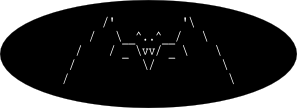
\includegraphics{Batman_logo.png}

Ausgehend von den Erfahrungen mit Freifunk-OLSR begannen die Entwickler
aus der Freifunk-Community im M"arz 2006 in Berlin damit, ein neues
Routingprotokoll f"ur drahtlose Meshnetzwerke zu entwickeln. Alle bisher
bekannten Routingalgorithmen versuchen Routen entweder zu berechnen
(proaktive Verfahren) oder sie dann zu suchen, wenn sie gebraucht werden
(reaktive Verfahren). Das neue Protokoll B.A.T.M.A.N. 
(BETTER APPROACH TO MOBILE ADHOC NETWORKING) berechnet oder
sucht im Gegensatz zu diesen Protokollen keine Routen, es erfasst
lediglich, ob Routen zu anderen Knoten existieren und "uberwacht ihre
Qualit"at. Dabei interessiert es sich nicht daf"ur, wie eine Route verl"auft,
sondern ermittelt lediglich, "uber welchen direkten Nachbarn ein bestimmter
Netzwerkknoten am besten zu erreichen ist, und tr"agt diese Information
proaktiv in die Routingtabelle ein. 


\subsection{Existierende L"osungen und Projekte}

(TODO) Einbisschen Text zu jedem Projekt (googeln)

\begin{itemize}
\item FreiFunk \url{http://freifunk.net/wiki/Meshing}
\item OpenNet \url{http://wiki.opennet-initiative.de/index.php/Hauptseite}
\item \url{http://www-i4.informatik.rwth-aachen.de/mcg/projects/umic-mesh/} 
\item \url{http://umic-mesh.net/}
\item (TODO) Google..

\end{itemize}
